\documentclass[10pt]{article}
\usepackage{amsmath,amssymb,amsthm,amsfonts,hyperref,fancyhdr,graphicx,subfig,bbm,verbatim,float,microtype,multirow,array,titlesec}
\usepackage[export]{adjustbox}
\usepackage[dvipsnames]{xcolor}
\usepackage[left=2cm,right=2cm,top=2cm,bottom=2cm]{geometry}
\usepackage[none]{hyphenat}
\usepackage[justification=centering]{caption}
\graphicspath{{../figures/clean2/}}
\setlength{\parindent}{0cm}
\titleformat*{\section}{\Large\bfseries}
\titleformat*{\subsection}{\large\bfseries}

\newcommand{\R}{\mathbb{R}}
\newcommand{\1}{\mathbbm{1}}
\newcommand{\0}{\mathbf{0}}
\newcommand{\p}{\mathbb{P}}

\renewcommand{\baselinestretch}{1.2}
\newcolumntype{M}[1]{>{\raggedright}m{#1}}

\begin{document}
\begin{center}
\sc\Large Clean training set \\ {\small\today}
\end{center}
\vspace{10pt}

Training set = Hong Kong database + balanced B100' subset for 20\% class 1 samples. 
\begin{table}[H]
\centering
\begin{tabular}{|c|c|c|c|c|c|c|c|c|c|c|}
\hline
size & 5221 &4708 &3809 &2843 &1880 &1116 &583 &265 &118 &36 \\
\hline
class 1\% & 19.21\% &19.14\% &19.01\% &18.71\% &18.09\% &17.20\% &15.61\% &14.72\% &13.56\% &19.44\%\\
\hline
\end{tabular}
\end{table}
\begin{figure}[H]
    \centering
    \subfloat[Accuracy]{\includegraphics[width=9cm]{acc_size_log}}
    \\
    \subfloat[AUC]{\includegraphics[width=9cm]{auc_size_log}}
\end{figure}

\begin{figure}[H]
    \centering
    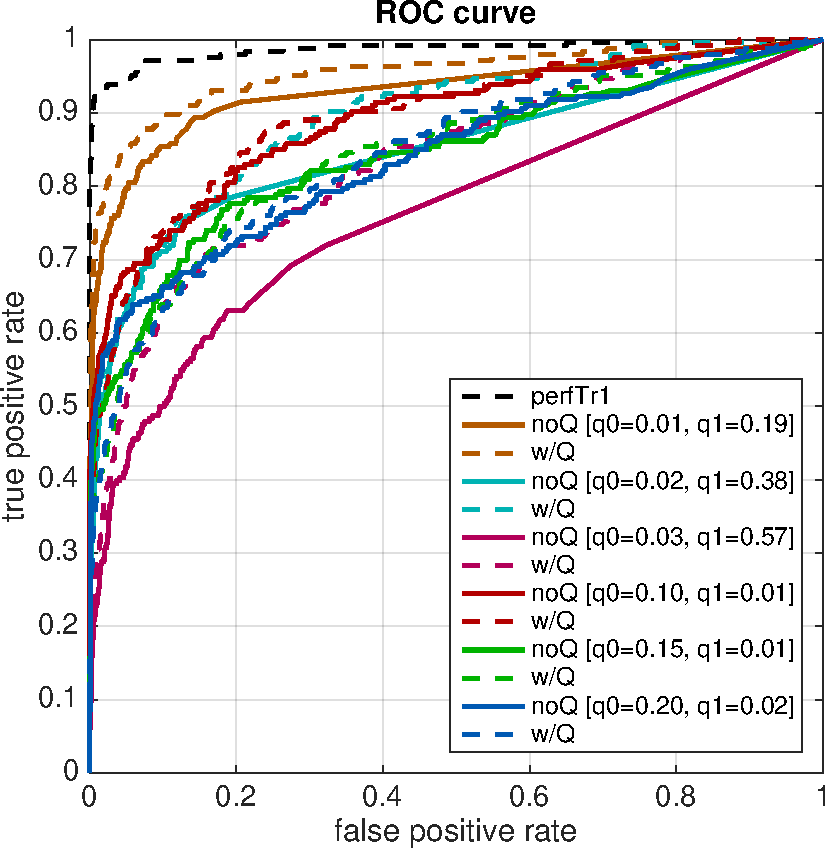
\includegraphics[width=9cm]{roc}
    \caption{ROC cruves}
\end{figure}

\begin{figure}[H]
    \centering
    \includegraphics[width=16cm]{auc_size_log_fus}
    \caption{AUC clean \& noisy}
\end{figure}
\end{document}